\documentclass[a4paper]{article}

%--------------------------------------------------------------------------
\usepackage[a4paper, total={6in, 9in}]{geometry}
\usepackage{amsmath}
\usepackage{booktabs}
\usepackage{caption}
\usepackage{enumitem}
\usepackage{graphicx}
\usepackage{float}
\usepackage{inconsolata}
\usepackage{listings}
\usepackage{pstricks-add}
\usepackage{siunitx}
\usepackage[most]{tcolorbox}
\usepackage{tikz}

\usetikzlibrary{shapes.geometric}

%--------------------------------------------------------------------------
\graphicspath{{./fig/}}

\begin{document}
\title{Udacity: 3D Perception Report}
\author{Shane Reynolds}
\maketitle
\section{Introduction \& Background}
In order for a robot to perform meaningful actions it requires some capacity to perceive its environment - the devices used to capture data about an environment are called sensors. There are two main categories into which sensors fall into: active, and passive. The principal distinction between these two types of sensors are that passive sensors measure energy which is already present in the environment, whilst active sensors emit some form of energy and measure the reactions of this energy with the environment. Table 1 (over the page) shows some examples of the more common sensors which are used for robotic perception. Generally, robotic perception systems are comprised of both active and passive sensors. In fact, both active and passive sensors are often combined into a single sensor to create a hybrid sensor. An example of a widely used hybrid sensor which features in many households is the Microsoft Kinect, shown in Figure 1.

\begin{figure}[h]
\centering
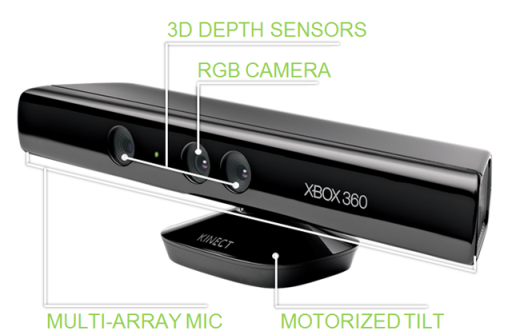
\includegraphics[scale=0.3]{image1}
\caption{The Microsoft Kinect is an example of a hybrid sensor called an RGBD camera. It captures 2D pixel arrays in 3 colour channels, in addition to capturing depth information using structured infra-red light pattern.}
\end{figure}

This project explores the perception of an environment using a hybrid sensor called an RGBD camera. This type of sensor captures a 2D pixel array on red, green, and blue channels using a monocular camera. Further, the sensor captures depth information by measuring the deformation of reflections from structured infra-red (IR) light emitted into the environment. The sensor will be employed using a WillowGarage PR2 robot simulated using ROS, Gazebo, and Rviz. A real world image of the PR2 can be seen in Figure 2, and a close up of the robot's sensing hardware can be seen in Figure 3.

\begin{figure}[H]
\centering
\begin{minipage}[t]{0.45\linewidth}
\centering
\frame{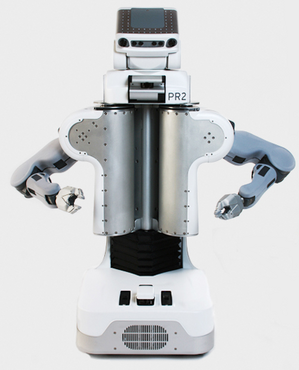
\includegraphics[height=3.3cm]{image2}}
\caption{A picture of the WillowGarage PR2 robot.}
\end{minipage}
\hspace{0.5cm}
\begin{minipage}[t]{0.45\linewidth}
\centering
\frame{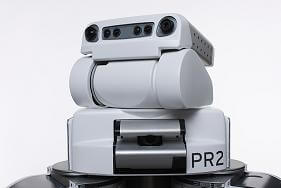
\includegraphics[height=3.3cm]{image3}}
\caption{A close up of the PR2's RGBD camera which captures image and depth data, and is used to create point clouds.}
\end{minipage}
\end{figure}

\begin{table}[h]
\centering
\caption{Examples of passive and active sensors which can be used for robotic perception systems (note that this list is not exhaustive)}
\begin{tabular}{p{2.3cm}p{4.5cm}p{2.3cm}p{4.5cm}}
\toprule
\multicolumn{2}{c}{\textbf{Passive Sensors}} & \multicolumn{2}{c}{\textbf{Active Sensors}}\\
\cmidrule(lr){1-2} \cmidrule(lr){3-4}
\textbf{Name} & \textbf{Description} & \textbf{Name} & \textbf{Description}\\
\midrule
Monocular Camera & A single RGB camera providing information on texture and shape & LIDAR & A 3D laser scanner which determines information about an environment through reading pulsed laser emission reflections\\
& & & \\
Stereo Camera & Consists of 2 monocular cameras providing the same information as the single monocular camera, but with the addition of depth information too & Time of Flight Camera & A 3D ToF camera performs depth measurement by illuminating environment with infra-red and observing the time taken to reflect from surfaces to the camera\\
& & & \\
& & Ultrasonic & Provides depth information by sending out high-frequency sound pulses and measuring time taken for sound to reverberate\\
\bottomrule
\end{tabular}
\end{table}

The captured sensor information is processed into a point cloud using the \verb|pcl| library which is implemented in ROS. Perception of an environment is not simply the capture of point cloud data, rather, it is the implementation of software in order to make sense of the point cloud data. The ultimate goal of this project is for the PR2 to identify objects on a table, pick these objects in a specified order, and stow them into the desired container either on the left or the right of the robot. In order to complete this task, there are two main sub-tasks that the robot's perception architecture must achieve: Segmentation, and Object Recognition. Segmentation is a complex process made up of many subtasks. Briefly, the segmentation implementation for this project is made up of the following sequence of activities:
\begin{enumerate}
\item Statistical filtering;
\item Voxel downsampling;
\item RANSAC plane filtering;
\item Passthrough filtering; and
\item Euclidean clustering (DBSCAN)
\end{enumerate}

Object



\newpage

\section{Methods \& Implementation}
\subsection{Segmentation}
\subsubsection{Obtain the Point Cloud}
The point cloud is obtained using an RGBD camera to capture a 2D image which consists of three feature maps, and a depth representation. The three feature maps represent the individual Red, Green, and Blue (RBG) channels for colour image. Each discrete pixel in the 2D array is also assigned an image depth. There are a total of 4 dimensions for each individual point cloud, which is assembled for use in the ROS environment by the pcl library.
 
***Add additional notes about structured light from RGBD camera***

***Tighten this up a little bit - look at algorithm and implementation***

\subsubsection{Statistical Filtering to Remove Image Noise}
The captured point cloud is not a perfect representation of the environment, rather, there are elements of noise introduced through XXXX (how is the noise introduced?). Noise is introduced to the image through dust in the environment and imperfect instrumentation. The noisy signal can be seen in Figure XXXX. A signal which has had noise removed can be seen in Figure XX. Why is the presence of noise in the point cloud a problem? The successful implementation of this vision system relies on clean segmentation of objects in a frame. The presence of noise results in the confusion of the segmentation alogrithm which is a Euclidean clustering method based on the DBSCAN algorithm.

***Need to tighten up on this paragraph***

\begin{figure}[h]
\begin{minipage}{0.45\linewidth}
\centering
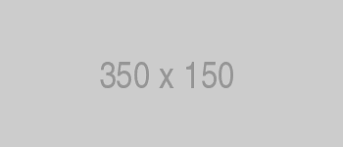
\includegraphics[scale=0.5]{placeholder}
\caption{include a figure - which shows the noisy image data}
\end{minipage}
\hspace{0.5cm}
\begin{minipage}{0.45\linewidth}
\centering
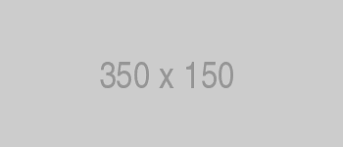
\includegraphics[scale=0.5]{placeholder}
\caption{include a figure which shows the noise present in a signal }
\end{minipage}
\end{figure}

\subsubsection{Voxel Downsampling}
Point clouds often provide more data than necessary to achieve an accurate representation of the robot environment. The processing of this data, left unchecked, is computationally expensive. Downsampling is the process of removing data points in a systematic fashion and is a technique that is often employed in the field of image processing. Voxel downsampling is analogous to this process - points in the three dimensional point cloud model are removed in a systematic fashion. Care needs to be taken when adjusting the parameters for the Voxel downsampling - if the downsampling is too aggressive too much information may be removed compromising the integrity of the pointcloud ***there may be a better way to say this - compromising an image looks like removing so much data that segmentation cannot occur successfully***

\begin{figure}[h]
\begin{minipage}{0.45\linewidth}
\centering
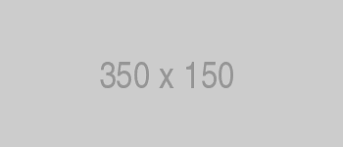
\includegraphics[scale=0.5]{placeholder}
\caption{include a figure which shows no Voxel Downsampling}
\end{minipage}
\hspace{0.5cm}
\begin{minipage}{0.45\linewidth}
\centering
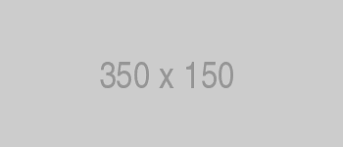
\includegraphics[scale=0.5]{placeholder}
\caption{include a figure which shows the basics of Voxel Downsampling}
\end{minipage}
\end{figure}

\subsubsection{RANSAC Plane Segmentation}
Random sample consensus (RANSAC) is an segmentation algorithm which detects statistical outliers according to some mathematical model. In this instance the mathematical model being used is a plane, which most closely resembles the table in the point cloud image. The model outliers, that is those points which don't statistically fit the mathematical representation of a plane, are filtered from the point cloud. The filtered points are stored in the variable ***look up the variable which the points are stored in***. This processing helps to isolate the objects in the image, ready for segmentation and object recognition.

***Need to reword this better***

Why is this a problem? Including the table in the point cloud image has the potential to confuse the Euclidean clustering algorithm since the segmentation is based on spatial proximity. Further benefits include the decreased computation cost for processing the remainder of the point cloud.

\begin{figure}[h]
\begin{minipage}{0.45\linewidth}
\centering
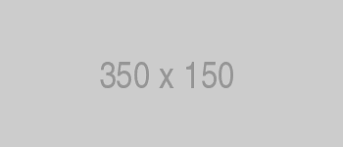
\includegraphics[scale=0.5]{placeholder}
\caption{Include an image of filtered point cloud table}
\end{minipage}
\hspace{0.5cm}
\begin{minipage}{0.45\linewidth}
\centering
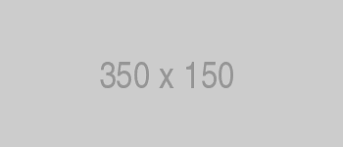
\includegraphics[scale=0.5]{placeholder}
\caption{Include an image of the filtered point cloud which has all of the objects only}
\end{minipage}
\end{figure}

\subsubsection{Passthrough Filtering}
A pass through filter is a simple filter designed to remove points from the point cloud which fall outside a spatially bounded region. This filter is very basic in its implementation, and does not rely on any statistical filters to achieve the results. In this instance, we remove points based which don't fall within an area bounded by a rectangular prism. Whilst not essential, to the overall processing this stops the robot from segmenting points which belong to the the boxes which lie to the left and the right of the work space, and removes the robot's arms from the point cloud.

\begin{figure}[h]
\begin{minipage}{0.45\linewidth}
\centering
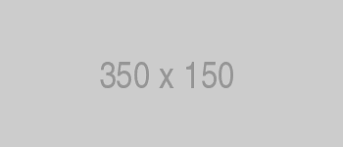
\includegraphics[scale=0.5]{placeholder}
\caption{Include and image of the unfiltered point cloud}
\end{minipage}
\hspace{0.5cm}
\begin{minipage}{0.45\linewidth}
\centering
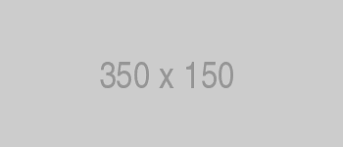
\includegraphics[scale=0.5]{placeholder}
\caption{Include an image of the filtered point cloud}
\end{minipage}
\end{figure}

\subsubsection{Euclidean Clustering (DBSCAN)}
Segmentation is important to implement successful object recognition. The segmentation works grouping points in the point cloud together based on their proximity to each other.

Potential problems with this method. This method encounters problems if the objects are too close to each other. If the objects are too close to each other, then the Euclidean clustering method fails - the algorithm will think that the objects 

\subsection{Object Recognition}


\section{Results \& Conclusion}


\section{Further Enhancements}


\end{document}